\section{Kreisel}\label{kap:}
Im zweiten Teil des Experimentes wurde das Trägheitsmoment eines Kreisels bestimmt
\subsection{Methoden}
Zunächst wurde wurde der Durchmesser der Kugel, die Länge l, die Masse m und für drei verschiedene Positionen des Zusatzgewichtes die Kraft F.
Jede dieser Messungen (bis auf die der Masse) wurde je 5 mal durchgeführt (Gemessene Größen vgl. Abb. \ref{fig:Kreisel})
Die Längen  wurden mit einem Messschieber gemessen und die Masse mit einer Waage mit digitaler Anzeige.
\begin{figure}[h]
	\centering
	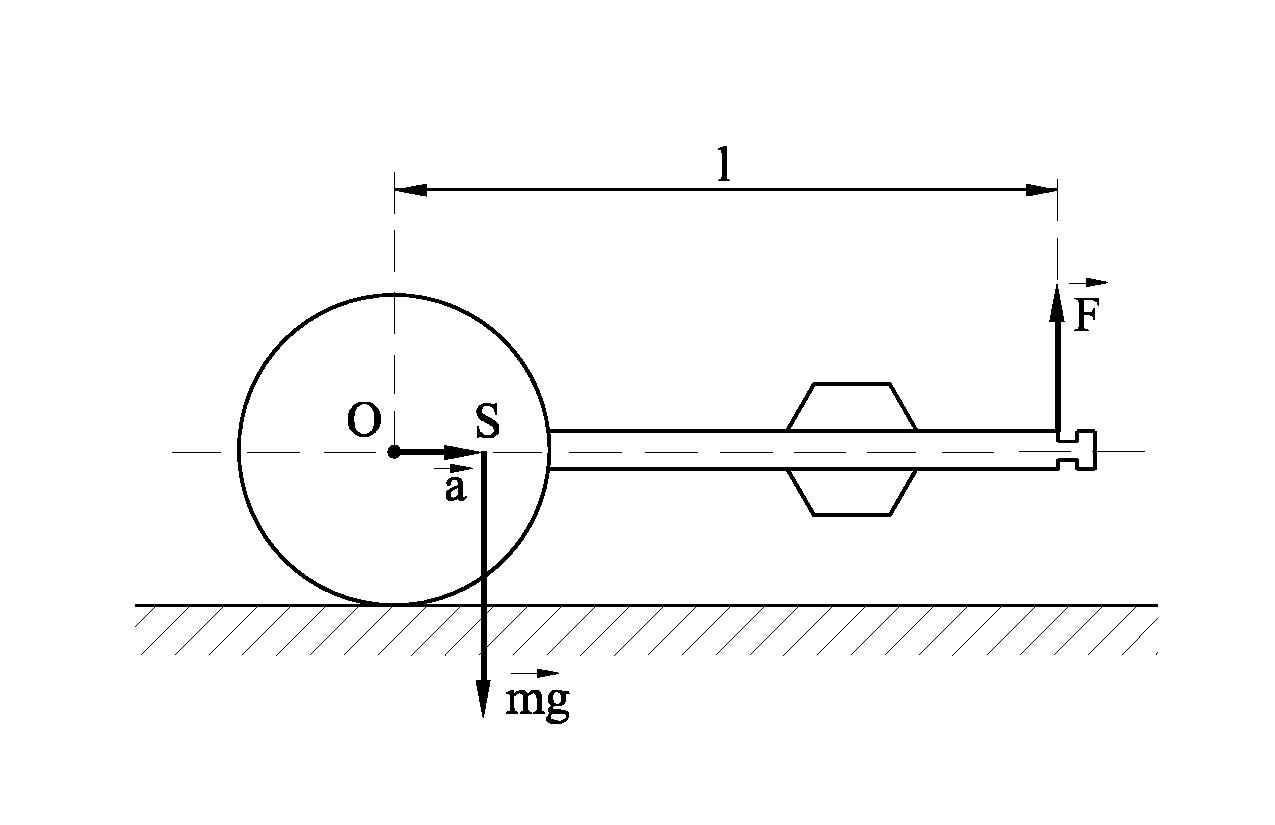
\includegraphics[width=0.7\linewidth]{res/KreiselAufbau.pdf}
	\caption{Schematische Darstellung des Kreisels bei Messung der Kraft F}
	\label{fig:kreisel}
\end{figure}
Mithilfe dieser Werte und dem aus der Anleitung gegeben Trägheitsmoment $J_{Stange}+J_{Zusatz}=\SI{15}{g cm^2}$ und den Formeln $J_{ges}=J_{Kugel}+J_{Stange}+J_{Zusatz}$ und $J_{Kugel}=\frac{2}{5}mr^2$ wurde der in \cref{kap:Zusammenfassung} schon genannte Wert für $J_{theo.}=\SI{1,3356+-0,0004e-4}{kg \cdot m^2}$ berechnet. Ein anderer Weg das Trägheitsmoment zu bestimmen war es diesen über den Zusammenhang zwischen l $\cdot$ F und  $\frac{\Delta \omega}{\Delta T_p}$ sowie dem Trägheitsmoment J. Um diesen Zusammenhang zu erhalten wurde die Präzessionszeit $T_p$ des Kreisels für drei Unterschiedliche Positionen des Zusatzgewichtes bei fünf unterschiedlichen Frequenzen gemessen. Einmal unten, einmal Mittig und einmal oben(Position 1,2 und 3). Zur Messung der Frequenz des Kreisels wurde der Kreisel mit einem Stroboskop beleuchtet. Die Frequenz des Stroboskops wurde als erstes eingestellt und der Kreisel wurde solange beschleunigt bis er die gleiche Frequenz hatte wie das Stroboskop.
Das der Kreisel die gleiche Frequenz erreicht hatte wie das Stroboskop wurde durch eine Markierung auf der Kugel des Kreisels ersichtlich. Sobald diese Markierung nahezu stillstand war die Frequenz erreicht. Es war jedoch nicht möglich zu verhindern das sich diese Markierung weiterbewegte. Da die Markierung sich jedoch sowohl mit der Drehbewegung bewegte als auch in die entgegengesetzte Richtung wurde bei den Rechnungen davon ausgegangen das sich diese entgegengesetzten Bewegungen in etwa aufheben. Die Präzessionzeit $T_p$ wurde gemessen indem der Kreisel leicht gekippt wurde und die Zeit für mehrere Umdrehungen der Stange gemessen wurde. Um die Winkelgeschwindigkeit $\omega$ zu erhalten wurde die Frequenz mit $2 \pi$ Multipliziert.
Die Präzessionszeit wurde dann für jede Position des Zusatzgewichtes gegen die Winkelgeschwindigkeit aufgetragen. Die Messwerte wurde mit einem linearen Fit genähert und das Produkt l $\cdot$ F wurde gegen den Kehwert der drei Steigungen aufgetragen. Die Steigung des Linearen Fits mit dem diese drei Punkte genähert wurde entspricht $J \cdot 2 \pi$.